\chapter{完成工作池应用程序}\label{chapt:worker-pool}

本章内容包括:

\begin{enumerate}
	\item 实现完整的工作池应用程序
  \item 构建多个监督层级
  \item 动态创建监督者和工作者
\end{enumerate}

在本章中,我们将继续发展在第 6 章开始的 \texttt{Pooly}的设计。
到本章结束时,我们将拥有一个完整且功能齐全的工作池应用程序。
我们将更深入地探索Supervisor API,并探讨更高级(也就是更有趣!)的监督者主题。

在第\ref{chapt:fault-tolerent}章中,我们停留在一个非常基础的工作池应用程序阶段,如果可以这样说的话。
在接下来的部分中,我们将为\texttt{Pooly}添加一些智能。
例如,目前还没有办法优雅地处理崩溃和重启。\texttt{Pooly}的当前版本只能处理单个池和固定数量的工作者。
第 3 版本的\texttt{Pooly}将实现对多个池的支持,以及对可变数量的工作进程的支持。

有时池需要处理意外负载。当请求太多时会发生什么?当所有工作者都忙时会发生什么?
在第4 版中,我们使池具有可变大小,允许工作者的\emph{溢出}。
我们还实现了在所有工作者都忙时对消费者进程的排队。

\section{版本3:错误处理、多个池和工作者}

我们如何知道一个进程崩溃了?我们可以监视或链接它。这引出了下一个问题,我们应该选择哪一个?为了回答这个问题,我们必须思考当进程崩溃时应该发生什么。有两种情况需要考虑。崩溃可能发生在:

· 服务器进程和消费者进程之间

· 服务器进程和工作者进程之间


\subsection{情况1:服务器和工作者之间的崩溃}

服务器进程的崩溃不应该影响消费者进程。事实上,反之亦然!当消费者进程崩溃时,它不应该使服务器进程崩溃。因此,\emph{监视器}
是正确的选择。

每次工作者检出时,我们已经在监视消费者进程。剩下的就是处理消费者进程的\texttt{:DOWN} 消息:

\begin{code}{lib/pooly/server.ex – 处理消费者进程的 :DOWN 消息}

\begin{minted}[linenos]{elixir}
defmodule Pooly.Server do
  #############
  # Callbacks #
  #############

  def handle_info({:DOWN, ref, _, _, _}, state = %{monitors: monitors, workers: workers}) do
    case :ets.match(monitors, {:"$1", ref}) do
      [[pid]] ->
        true = :ets.delete(monitors, pid)
        # 1
        new_state = %{state | workers: [pid | workers]}
        {:no_reply, new_state}

      [[]] ->
        {:no_reply, state}
    end
  end
end

# 1 将工作者返回到池中
\end{minted}
\label{lst:worker-pool-handle-info}
\end{code}

当消费者进程崩溃时,我们在 \texttt{monitors} ETS表中匹配引用,删除监视器,并将工作者添加回状态中。


\subsection{情况2:服务器和工作者之间的崩溃}

如果服务器崩溃,它应该带下工作者进程吗?应该,因为否则,服务器的状态将与池的实际状态不一致。
另一方面,当工作者进程崩溃时,它应该使服务器进程崩溃吗?当然不是!这对我们意味着什么?
嗯,由于双向依赖,我们应该使用\emph{链接}。然而,由于服务器在工作者进

程崩溃时 \emph{不应} 崩溃,服务器进程应该捕获退出:

\begin{code}{}
\begin{minted}[linenos]{elixir}
defmodule Pooly.Server do
  #############
  # Callbacks #
  #############
  def init([sup, pool_config]) when is_pid(sup) do
    # 1
    Process.flag(:trap_exit, true)
    monitors = :ets.new(:monitors, [:private])
    init(pool_config, %State{sup: sup, monitors: monitors})
  end
end

# 1 设置服务器进程以捕获退出。
\end{minted}
% \label{lst:id}
\end{code}

现在服务器进程已经开始捕获退出,我们应该处理来自工作者的
\texttt{:EXIT} 消息:

\begin{code}{}
\begin{minted}[linenos]{elixir}
defmodule Pooly.Server do
  #############
  # Callbacks #
  #############

  def handle_info(
        {:EXIT, pid, _reason},
        state = %{monitors: monitors, workers: workers, worker_sup: worker_sup}
      ) do
    case :ets.lookup(monitors, pid) do
      [{pid, ref}] ->
        true = Process.demonitor(ref)
        true = :ets.delete(monitors, pid)
        new_state = %{state | workers: [new_worker(worker_sup) | workers]}
        {:noreply, new_state}

      [[]] ->
        {:noreply, state}
    end
  end
end
\end{minted}
% \label{lst:id}
\end{code}

当工作者进程意外退出时,在 \texttt{monitors} ETS
表中查找其条目。如果条目不存在,则无需执行任何操作。否则,不再监视消费者进程,并从
\texttt{monitors}
表中删除其条目。最后,创建一个新的工作者并将其添加回服务器状态的工作者字段中。

 \subsection{ 处理多个池}

在第 2
版之后,我们有了一个非常基本的工作池。然而,任何自尊的工作池应用程序都应该能够处理多个池。在我们开始编码之前,让我们先考虑一些可能的设计。最直接的方法是这样设计监督树:

\begin{figure}[!ht]
    \centering
    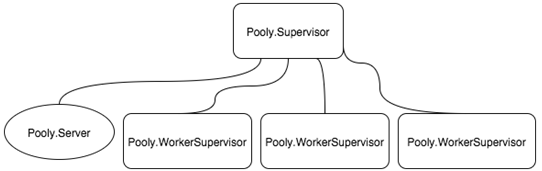
\includegraphics[width=0.8\linewidth]{7_1.png}
    \caption{处理多个池的可能设计}
    \label{fig:7_1}
\end{figure}


你看到问题了吗?我们实际上是在
\texttt{Pooly.Supervisor} 中添加更多的
\texttt{WorkerSupervisor}。这是一个糟糕的设计。问题在于
\emph{错误核心},或者说缺乏错误核心。

请允许我详细说明。任何 \texttt{WorkerSupervisor}
的问题都不应该影响
\texttt{Pooly.Server}。思考当一个进程崩溃时会发生什么,以及谁会受到影响是值得的。一个潜在的修复方法可能是添加另一个监督者来处理所有工作者监督者,比如
\texttt{Pooly.WorkersSupervisor}(\emph{只是}
另一个间接层!)。现在它可能是这样的:

\begin{figure}[!ht]
    \centering
    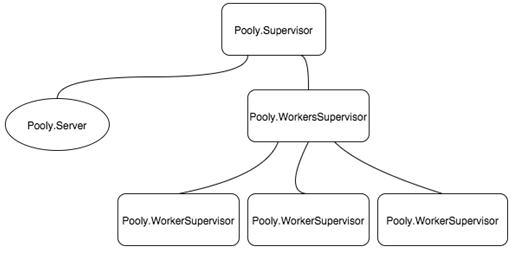
\includegraphics[width=0.8\linewidth]{7_2.png}
    \caption{另一种可能的设计。你能识别出瓶颈吗?}
    \label{fig:7_2}
\end{figure}


你注意到另一个问题了吗?可怜的 \texttt{Pooly.Server}
必须处理 \emph{每个}
池的所有请求。这意味着如果消息快速而猛烈地发送到服务器进程,可能会导致服务器进程成为瓶颈,并可能淹没其邮箱。\texttt{Pooly.Server}
也是单点故障,因为它包含每个池的状态。服务器进程的死亡意味着 \emph{所有}
工作者监督者都必须被关闭。那么考虑一下这个设计:

\begin{figure}[!ht]
    \centering
    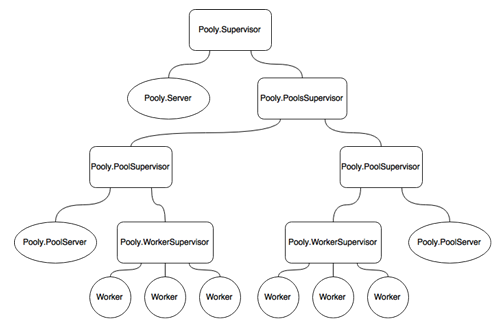
\includegraphics[width=0.8\linewidth]{7_3.png}
    \caption{Pooly 的最终设计}
    \label{fig:7_3}
\end{figure}



\subsubsection{顶层监督器}

\texttt{Pooly.Supervisor} 作为顶层监督器,管理一个
\texttt{Pooly.Server} 和一个
\texttt{PoolsSupervisor}。\texttt{PoolsSupervisor}
又管理多个 \texttt{PoolSupervisor}。每个
\texttt{PoolSupervisor} 管理自己的
\texttt{PoolServer} 和
\texttt{WorkerSupervisor}。

如你所猜测的,Pooly将进行设计大修。为了便于跟踪,我们将从上到下实施更改。


\subsection{添加应用行为到 Pooly}

首先要更改的地方是
\texttt{lib/pooly.ex},Pooly的主入口。由于我们现在支持多个池(pool),我们希望通过其名称引用每个池。这意味着各种函数也将接受
\texttt{pool\_name} 作为参数:


\subparagraph{代码 7.4 lib/pooly.ex -
添加对多个池的支持}

\begin{code}{}
\begin{minted}[linenos]{elixir}
defmodule Pooly do
  use Application

  def start(_type, _args) do
    # 2
    # 1
    pools_config =
      [
        # 1
        [
          name: "Pool1",
          # 1
          mfa: {SampleWorker, :start_link, []},
          size: 2
        ],
        # 1
        [
          name: "Pool2",
          # 1
          mfa: {SampleWorker, :start_link, []},
          size: 3
        ],
        # 1
        [
          name: "Pool3",
          # 1
          mfa: {SampleWorker, :start_link, []},
          size: 4
        ]
      ]

    # 1

    # 2
    start_pools(pools_config)
  end

  # 2
  def start_pools(pools_config) do
    # 2
    Pooly.Supervisor.start_link(pools_config)
  end

  # 3
  def checkout(pool_name) do
    # 3
    Pooly.Server.checkout(pool_name)
  end

  # 3
  def checkin(pool_name, worker_pid) do
    # 3
    Pooly.Server.checkin(pool_name, worker_pid)
  end

  # 3
  def status(pool_name) do
    # 3
    Pooly.Server.status(pool_name)
  end
end

# 1 池配置现在接受多个池的配置。池也有名称。
# 2 从 pool\_config 到 pools\_config 的复数变化。
# 3 其余的 API 接受 pool\_name 作为参数。
\end{minted}
% \label{lst:id}
\end{code}




\subsection{添加顶层监督器}

我们的下一站是顶层监督器,\texttt{lib/pooly/supervisor.ex}。顶层监督器负责启动
\texttt{Pooly.Server} 和
\texttt{Pooly.PoolsSupervisor}。当
\texttt{Pooly.PoolsSupervisor} 启动时,它启动各自的
\texttt{Pooly.PoolSupervisor},而这些又启动它们自己的
\texttt{Pooly.Server} 和
\texttt{Pooly.WorkerSupervisor}。


\begin{figure}[!ht]
    \centering
    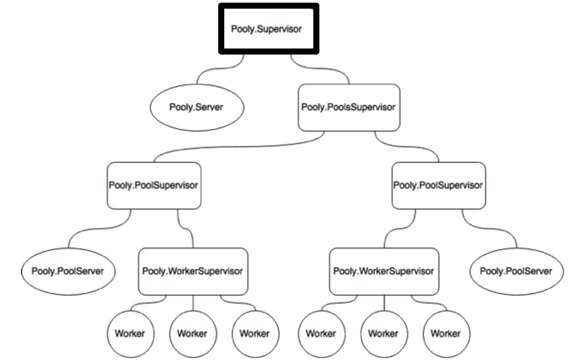
\includegraphics[width=0.8\linewidth]{7_4.png}
    \caption{从顶层监督器开始}
    \label{fig:7_4}
\end{figure}


看图,\texttt{Pooly.Supervisor}
监督两个进程:\texttt{Pooly.PoolsSupervisor}(尚未实现)和
\texttt{Pooly.Server}。因此,我们需要将这两个进程添加到
\texttt{Pooly.Supervisor}
的子进程列表中。我们就这样做:


\subparagraph{代码 7.5 lib/pooly/supervisor.ex --
顶层监督器监督顶层池服务器和池监督器}

\begin{code}{}
\begin{minted}[linenos]{elixir}
defmodule Pooly.Supervisor do
  use Supervisor

  def start_link(pools_config) do                       #1
    Supervisor.start_link(__MODULE__, pools_config,
                          name: __MODULE__)             #2
  end

  def init(pools_config) do                             #1
    children = [
      supervisor(Pooly.PoolsSupervisor, []),            #3
      worker(Pooly.Server, [pools_config])              #3
    ]

    opts = [strategy: :one_for_all]

    supervise(children

, opts)
  end
end

#1 从 pool\_config 到 pools\_config 的复数变化。
#2 Pooly.Supervisor 现在是一个命名进程。
#3 Pooly.Supervisor 现在监督两个子进程。注意 Pooly.Server 不再需要Pooly.Supervisor 的 pid,因为我们可以通过名称引用它。
\end{minted}
% \label{lst:id}
\end{code}

\texttt{Pooly.Supervisor} 的主要变化是添加
\texttt{Pooly.PoolsSupervisor} 作为子进程,并给
\texttt{Pooly.Supervisor} 命名。回想一下,我们在 \#1
中将 \texttt{Pooly.Supervisor} 的名称设置为
\texttt{\_\_MODULE\_\_},这意味着我们可以将进程引用为
\texttt{Pooly.Supervisor} 而不是
pid。因此,我们不需要将 \texttt{self}(参见
\texttt{Pooly.Supervisor} 的第二版)传递给
\texttt{Pooly.Server}。


\subsection{添加池的监督器}

在 \texttt{lib/pooly/} 下创建
\texttt{pools\_supervisor.ex}。以下是实现:


\subparagraph{代码 7.6 lib/pooly/pools\_supervisor.ex --
池监督器的完整实现}

\begin{code}{}
\begin{minted}[linenos]{elixir}
defmodule Pooly.PoolsSupervisor do
  use Supervisor

  def start_link do
    # 1
    Supervisor.start_link(__MODULE__, [], name: __MODULE__)
  end

  def init(_) do
    opts = [
      # 2
      strategy: :one_for_one
    ]

    supervise([], opts)
  end
end
\end{minted}
% \label{lst:id}
\end{code}

就像 \texttt{Pooly.Supervisor},我们给
\texttt{Pooly.PoolsSupervisor}
命名。注意这个监督器没有子规格。事实上,当它启动时,没有任何池附加到它。这是因为,就像版本
2
一样,我们想在创建任何池之前验证池配置。因此,我们提供的唯一信息是重启策略,如
\#2 所示。为什么是
\texttt{:one\_for\_one}?任何池的崩溃都不应该影响其他池。

\subsection{使 Pooly.Server 更简单}

在第一版和第二版中,我们说 \texttt{Pooly.Server}
是整个操作的大脑。但现在不再是这样了。\texttt{Pooly.Server}
的一些工作将由专门的 \texttt{Pooly.PoolServer} 接管。

\begin{figure}[!ht]
\centering
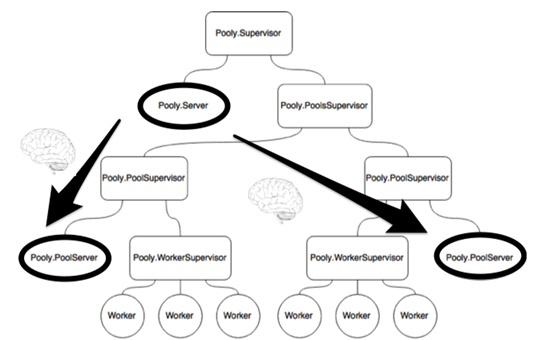
\includegraphics[width=0.8\linewidth]{7_6.png}
\caption{从之前版本的顶级池服务器中移动的逻辑将被移至各个池服务器}
\end{figure}

图 7.6 从之前版本的顶级池服务器中移动的逻辑将被移至各个池服务器

大多数 API 与之前版本相同,增加了
\texttt{pool\_name}。打开
\texttt{lib/pooly/server.ex}
并\emph{替换}之前的实现为以下内容:

\begin{code}{lib/pooly/server.ex - 顶级池服务器的完整实现}

\begin{minted}[linenos]{elixir}
defmodule Pooly.Server do
  use GenServer
  import Supervisor.Spec

  ####### 
  # API #
  #######

  def start_link(pools_config) do
    GenServer.start_link(__MODULE__, pools_config, name: __MODULE__)
  end

  def checkout(pool_name) do
    # 2
    GenServer.call(:"#{pool_name}Server", :checkout)
  end

  def checkin(pool_name, worker_pid) do
    # 2
    GenServer.cast(:"#{pool_name}Server", {:checkin, worker_pid})
  end

  def status(pool_name) do
    # 2
    GenServer.call(:"#{pool_name}Server", :status)
  end

  #############
  # Callbacks #
  #############

  # 3
  def init(pools_config) do
    # 3
    pools_config
    |> Enum.each(fn pool_config ->
      # 3
      send(self, {:start_pool, pool_config})
    end)

    # 3

    {:ok, pools_config}
  end

  # 4
  def handle_info({:start_pool, pool_config}, state) do
    # 4
    {:ok, _pool_sup} = Supervisor.start_child(Pooly.PoolsSupervisor, supervisor_spec(pool_config))
    {:no_reply, state}
  end

  #####################
  # Private Functions #
  #####################

  defp supervisor_spec(pool_config) do
    # 5
    opts = [id: :"#{pool_config[:name]}Supervisor"]
    supervisor(Pooly.PoolSupervisor, [pool_config], opts)
  end
end
\end{minted}
% \label{lst:id}
\end{code}

在这个版本中,\texttt{Pooly.Server}
的工作是\emph{委托}所有请求给相应的池,并启动池并将池附加到
\texttt{Pooly.PoolsSupervisor}。

在 \#2 中,我们假设每个单独的池服务器被命名为
\texttt{:"\#\{pool\_name\}Server"}。注意名字是\emph{原子}!遗憾的是,因为我未能正确阅读文档,我在这上面浪费了几个小时(和头发)。

在 \#3 中,\texttt{pools\_config} 被迭代,发送
\mintinline{elixir}|{:start_pool, pool\_config}| 消息给自己。在
\#4 中处理消息,告诉 \texttt{Pooly.PoolsSupervisor}
根据给定的 \texttt{pool\_config} 启动一个子进程。

这里有一个\emph{微小}的注意点。注意在 \#5 中我们确保每个
\texttt{Pooly.PoolSupervisor} 以\emph{独特}的监督器规范
id 启动。如果忘记这样做,你会得到一个如下的神秘错误信息:

\begin{code}{}
\begin{minted}[linenos]{elixir}
12:08:16.336 [error] GenServer Pooly.Server terminating
Last message: {:start_pool, [name: "Pool2", mfa: {SampleWorker, :start_link, []}, size: 2]}
State: [[name: "Pool1", mfa: {SampleWorker, :start_link, []}, size: 2], [name: "Pool2", mfa: {SampleWorker, :start_link, []}, size: 2]]
** (exit) an exception was raised:
** (MatchError) no match of right hand side value: {:error, {:already_started, #PID<0.142.0>}}
(pooly) lib/pooly/server.ex:38: Pooly.Server.handle_info/2
(stdlib) gen_server.erl:593: :gen_server.try_dispatch/4
(stdlib) gen_server.erl:659: :gen_server.handle_msg/5
(stdlib

) proc_lib.erl:237: :proc_lib.init_p_do_apply/3
\end{minted}
% \label{lst:id}
\end{code}

这里的线索是
\mintinline{elixir}|{:error, \{:already_started, \#PID<0.142.0>\}}|。我花了几个小时试图解决这个问题,直到偶然发现这个解决方案。当一个
\texttt{Pooly.PoolSupervisor} 以给定的
\texttt{pool\_config} 启动时会发生什么?

\subsection{添加池监督器}

\begin{figure}[!ht]
    \centering
    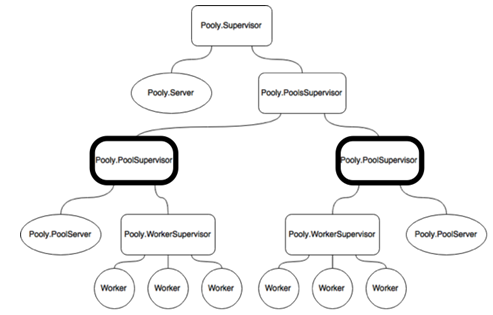
\includegraphics[width=0.8\linewidth]{7_7.png}
    \caption{实现各个池监督器}
    \label{fig:7_7}
\end{figure}

\texttt{Pooly.PoolSupervisor} 取代了之前版本的
\texttt{Pooly.Supervisor}。因此,只有一些小的更改。首先,每个
\texttt{Pooly.PoolSupervisor}
现在都初始化了一个名字。其次,我们需要告诉
\texttt{Pooly.PoolSupervisor} 使用
\texttt{Pooly.PoolServer}。以下是更改内容:

\begin{code}{lib/pooly/pool\_supervisor.ex - 单个池监督器的完整实现}

\begin{minted}[linenos]{elixir}
defmodule Pooly.PoolSupervisor do
  use Supervisor

  def start_link(pool_config) do
    # 1
    Supervisor.start_link(__MODULE__, pool_config, name: :"#{pool_config[:name]}Supervisor")
  end

  def init(pool_config) do
    opts = [
      strategy: :one_for_all
    ]

    children = [
      # 2
      worker(Pooly.PoolServer, [self, pool_config])
    ]

    supervise(children, opts)
  end
end
\end{minted}
% \label{lst:id}
\end{code}

我们在 \#1
中给单个池监督器命名,尽管这并非严格必要。这有助于我们在观察器中轻松找到池监督器。

其次,\#2 中的子进程规范从 \texttt{Pooly.Server} 更改为
\texttt{Pooly.PoolServer}。我们传递相同的参数。尽管我们正在命名
\texttt{Pooly.PoolSupervisor},我们将\emph{不会}在
\texttt{Pooly.PoolServer}
中使用该名称,这样我们可以重用来自版本2的
\texttt{Pooly.Server} 的大部分实现。


\subsection{添加池(Pool)的核心逻辑}

如上一节所述,大部分逻辑保持不变,只是在一些地方进行了修改以支持多个池。为了节约纸张和屏幕空间,与\texttt{Pooly.Server}版本2完全相同的函数被用``\texttt{\# …}''标记了出来。换句话说,如果你在跟随学习,可以将\texttt{Pooly.Server}版本2的实现复制粘贴到\texttt{Pooly.PoolyServer}。

以下是\texttt{Pooly.PoolServer}的实现:



\begin{code}{代码 7.9 lib/pooly/pool\_server.ex -单个池服务器的完整实现}

\begin{minted}[linenos]{elixir}
defmodule Pooly.PoolServer do
  use GenServer
  import Supervisor.Spec

  defmodule State do
    defstruct pool_sup: nil,
              worker_sup: nil,
              monitors: nil,
              size: nil,
              workers: nil,
              name: nil,
              mfa: nil
  end

  def start_link(pool_sup, pool_config) do
    GenServer.start_link(__MODULE__, [pool_sup, pool_config], name: name(pool_config[:name]))
  end

  def checkout(pool_name) do
    GenServer.call(name(pool_name), :checkout)
  end

  def checkin(pool_name, worker_pid) do
    GenServer.cast(name(pool_name), {:checkin, worker_pid})
  end

  def status(pool_name) do
    GenServer.call(name(pool_name), :status)
  end

  # 回调函数
  # ...

  def init([pool_sup, pool_config]) when is_pid(pool_sup) do
    Process.flag(:trap_exit, true)
    monitors = :ets.new(:monitors, [:private])
    init(pool_config, %State{pool_sup: pool_sup, monitors: monitors})
  end

  def init([{:name, name} | rest], state) do
    # …
  end

  # 其他初始化函数
  # ...

  def handle_call(:checkout, {from_pid, _ref}, %{workers: workers, monitors: monitors} = state) do
    # …
  end

  def handle_call(:status, _from, %{workers: workers, monitors: monitors} = state) do
    # …
  end

  def handle_cast({:checkin, worker}, %{workers: workers, monitors: monitors} = state) do
    # …
  end

  def handle_info(
        :start_worker_supervisor,
        state = %{pool_sup: pool_sup, name: name, mfa: mfa, size: size}
      ) do
    {:ok, worker_sup} = Supervisor.start_child(pool_sup, supervisor_spec(name, mfa))
    workers = prepopulate(size, worker_sup)
    {:no_reply, %{state | worker_sup: worker_sup, workers: workers}}
  end

  def handle_info({:DOWN, ref, _, _, _}, state = %{monitors: monitors, workers: workers}) do
    # …
  end

  # 其他处理函数
  # ...

  def terminate(_reason, _state) do
    :ok
  end

  # 私有函数
  # ...

  defp name(pool_name) do
    :"#{pool_name}Server"
  end

  defp prepopulate(size, sup) do
    # …
  end

  # 其他预填充函数
  # ...

  defp supervisor_spec(name, mfa) do
    opts = [id: name <> "WorkerSupervisor", restart: :temporary]
    supervisor(Pooly.WorkerSupervisor, [self, mfa], opts)
  end
end
\end{minted}
% \label{lst:id}
\end{code}

这里有几个显著的变化。服务器的\texttt{start\_link/2}函数将\emph{池监督器}作为第一个参数。在\#3中,池监督器的pid被保存在服务器进程的状态中。此外,注意服务器的状态已扩展以存储池监督器和工作监督器的pid:

\begin{code}{}
\begin{minted}[linenos]{elixir}
defmodule State do
  defstruct pool_sup: nil,
            worker_sup: nil,
            monitors: nil,
            size: nil,
            workers: nil,
            name: nil,
            mfa: nil
end
\end{minted}
% \label{lst:id}
\end{code}

一旦服务器处理完池配置,它将最终向自己发送\texttt{:start\_worker\_supervisor}消息,如\#4所示。这条消息由\texttt{handle\_info/2}回调处理。在

\#5中,池监督器被告知作为子项启动工作监督器,使用\#8中定义的子进程规范。除了\texttt{mfa},我们还传递了服务器进程的pid。一旦返回工作监督器的pid,它就会在\#6中被用来预填充\texttt{Worker}。\#2利用\texttt{name/1}来引用适当的池服务器以调用相应的函数。

\subsection{为池添加工作监管器}

最后一部分是工作监管器。它负责管理单个工作程序。它管理任何崩溃的工作程序。有一个微妙的细节。在初始化期间,工作监管器创建了与其对应池服务器的\emph{链接}。为什么要这样做?如果池服务器或工作监管器中的任何一个停止工作,另一个继续存在就没有意义了。

\begin{figure}[!ht]
    \centering
    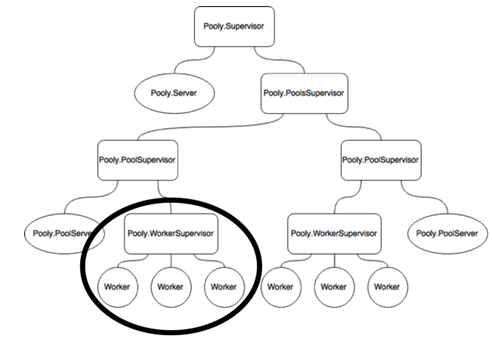
\includegraphics[width=0.8\linewidth]{7_8.png}
    \caption{实现单个池的工作监管器}
    \label{fig:7_8}
\end{figure}


让我们看看完整实现的更多细节:

代码代码 7.10 lib/pooly/worker\_supervisor.ex --
池的工作监管器的完整实现

\begin{code}{}
\begin{minted}[linenos]{elixir}
defmodule Pooly.WorkerSupervisor do
  use Supervisor

  # 1
  def start_link(pool_server, {_, _, _} = mfa) do
    # 1
    Supervisor.start_link(__MODULE__, [pool_server, mfa])
  end

  def init([pool_server, {m, f, a}]) do
    # 2
    Process.link(pool_server)
    worker_opts = [restart: :temporary, shutdown: 5000, function: f]

    children = [worker(m, a, worker_opts)]
    opts = [strategy: :simple_one_for_one, max_restarts: 5, max_seconds: 5]

    supervise(children, opts)
  end
end
\end{minted}
% \label{lst:id}
\end{code}

唯一的变化是增加了额外的\texttt{pool\_server}参数,并将\texttt{pool\_server}与工作监管器进程链接。为什么?如前所述,这两个进程之间存在依赖关系,当工作监管器停止工作时,需要通知池服务器。同样,如果工作监管器崩溃,它也应该同时带下池服务器。

为了让池服务器处理这个消息,你需要在\texttt{lib/pooly/pool\_server.ex}中添加另一个\texttt{handle\_info/2}回调:

代码代码 7.11 lib/pooly/pool\_server.ex --
让池服务器检测到工作监管器停止工作

\begin{code}{}
\begin{minted}[linenos]{elixir}
defmodule Pooly.PoolServer do
  #############
  # Callbacks #
  #############

  def handle_info({:EXIT, worker_sup, reason}, state = %{worker_sup: worker_sup}) do
    {:stop, reason, state}
  end
end
\end{minted}
% \label{lst:id}
\end{code}

在这里,每当工作监管器退出时,它也会终止池服务器,并且原因是与终止工作监管器的原因相同。

\subsection{将其实际运行}

让我们确保我们正确地连接了一切。首先,打开\texttt{lib/pooly.ex}来配置池。确保\texttt{start/2}函数看起来像这样:

代码\begin{code}{lib/pooly.ex -- 配置 Pooly 启动三个不同大小的池}

\begin{minted}[linenos]{elixir}
defmodule Pooly do
use Application

def start(_type, _args) do
pools_config =
[
[name: "Pool1", mfa: {SampleWorker, :start_link, []}, size: 2],
[name: "Pool2", mfa: {SampleWorker, :start_link, []}, size: 3],
[name: "Pool3", mfa: {SampleWorker, :start_link, []}, size: 4]
]

start_pools(pools_config)
end

# …end
\end{minted}
% \label{lst:id}
\end{code}

在这里,我们告诉 Pooly
创建三个池,每个池具有给定的大小和工作类型。为了简单(实际上是懒惰),我们在所有三个池中都使用了\texttt{SampleWorker}。在一个新的终端会话中,启动\texttt{iex}并启动
Observer:

\begin{code}{}
\begin{minted}[linenos]{elixir}
% iex -S mix
iex> :observer.start
\end{minted}
% \label{lst:id}
\end{code}

见证你所创建的壮丽监管树:

\begin{figure}[!ht]
    \centering
    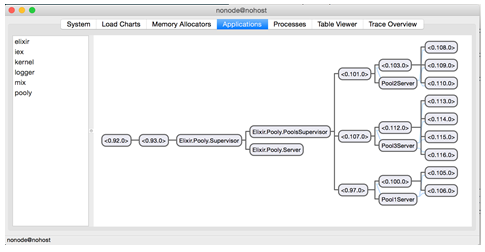
\includegraphics[width=0.8\linewidth]{7_9.png}
    \caption{从 Observer 看到的 Pooly 监管树}
    \label{fig:7_9}
\end{figure}


现在,从监管树的叶子(最低/最右边)开始,

尝试右击进程并杀死它。你会再次注意到一个新进程会接管。

接下来,往上走。比如,当杀死\texttt{Pool3Server}时会发生什么?你会注意到对应的\texttt{WorkerSupervisor}和它下面的工作程序都会被杀死并重新生成。重要的是要注意,\texttt{Pool3Server}是一个全新的进程。

现在再往上走。当你杀死一个\texttt{PoolSupervisor}时会发生什么?正如预期的那样,它下面的所有东西都会被杀死,另一个\texttt{PoolSupervisor}会重新生成,它下面的所有东西也会重新生成。注意不会发生的事情。应用程序的其余部分不会受到影响。这不是很棒吗?当崩溃发生时,正如它们不可避免地会发生的那样,拥有一个精心层次化的监管层次结构可以让错误以非常孤立的方式处理,从而不影响应用程序的其余部分。

\section{版本 4:实现溢出和排队功能}

在 Pooly
的最终版本中,我们将扩展它以支持可变数量的工作进程,方法是指定一个\emph{最大溢出量}。

我们还希望引入\emph{排队}工作进程的概念。也就是说,当达到最大溢出限制时,Pooly
能够为愿意\emph{阻塞并等待}下一个可用工作进程的消费者排队工作进程。

\subsection{实现最大溢出}

像往常一样,为了指定最大溢出,我们在池配置中添加了一个新字段。在
\texttt{lib/pooly.ex} 中,修改
\texttt{start/2} 中的
\texttt{pools\_config},使其看起来如下:

\begin{code}{lib/pooly.ex - 实现最大溢出}

\begin{minted}[linenos]{elixir}
defmodule Pooly do

def start(_type, _args) do
pools_config =
[
[name: "Pool1",
mfa: {SampleWorker, :start_link, []},
size: 2,
max_overflow: 3                       #1
],
[name: "Pool2",
mfa: {SampleWorker, :start_link, []},
size: 3,
max_overflow: 0                       #1
],
[name: "Pool3",
mfa: {SampleWorker, :start_link, []},
size: 4,
max_overflow: 0                       #1
]
]

start_pools(pools_config)
end
end
#1 在池配置中指定最大溢出。
\end{minted}
% \label{lst:id}
\end{code}


现在我们有了池配置的新选项,我们必须前往
\texttt{lib/pooly/pool\_server.ex} 以支持
\texttt{max\_overflow}。这包括:

· 在 \texttt{State} 中添加一个名为
\texttt{max\_overflow} 的条目

· 在 \texttt{State} 中添加一个名为
\texttt{overflow} 的条目,用于跟踪当前溢出计数

· 在 \texttt{init/2} 中添加一个函数子句来处理
\texttt{max\_overflow}

以下是添加内容:

\begin{code}{lib/pooly/pool\_server.ex - 在池服务器中添加最大溢出选项}

\begin{minted}[linenos]{elixir}
defmodule Pooly.PoolServer do
  defmodule State do
    defstruct pool_sup: nil,
              worker_sup: nil,
              monitors: nil,
              size: nil,
              workers: nil,
              name: nil,
              mfa: nil,
              overflow: nil,
              max_overflow: nil
  end

  #############
  # Callbacks #
  #############

  def init([{:name, name} | rest], state) do
    # …
  end

  # … more init/1 definitions

  def init([{:max_overflow, max_overflow} | rest], state) do
    init(rest, %{state | max_overflow: max_overflow})
  end

  def init([], state) do
    # …
  end

  def init([_ | rest], state) do
    # …
  end
end
\end{minted}
% \label{lst:id}
\end{code}

接下来,我们必须考虑实际溢出的情况。当忙碌工作进程的总数超过
\texttt{size} \emph{并且} 在
\texttt{max\_overflow}
限制内时,就会发生溢出。何时会发生溢出?当工作进程被\emph{取出}时。因此,唯一需要查看的地方是
\texttt{handle\_call(\{:checkout, block\}, from, state)}。

处理这种情况相当简单。\#1
检查我们是否在溢出限制内。如果是,将创建一个新的工作进程,并将必要的簿记信息添加到
\texttt{monitors} ETS 表中。然后将工作进程 pid
作为回复发送给消费者进程,并增加 \texttt{overflow}
计数:

\begin{code}{lib/pooly/pool\_server.ex - 在池服务器中处理取出时的溢出}

\begin{minted}[linenos]{elixir}
defmodule Pooly.PoolServer do
  #############
  # Callbacks #
  #############

  def handle_call({:checkout, block}, {from_pid, _ref} = from, state) do
    %{
      worker_sup: worker_sup,
      workers: workers,
      monitors: monitors,
      overflow: overflow,
      max_overflow: max_overflow
    } = state

    case workers do
      [worker | rest] ->
        # …
        {:reply, worker, %{state | workers: rest}}

      # 1
      [] when max_overflow > 0 and overflow < max_overflow ->
        {worker, ref} = new_worker(worker_sup, from_pid)
        true = :ets.insert(monitors, {worker, ref})
        {:reply, worker, %{state | overflow: overflow + 1}}

      [] ->
        {:reply, :full, state}
    end
  end
end
\end{minted}
% \label{lst:id}
\end{code}

\subsection{处理工作进程签入}

现在我们可以处理溢出了,那么我们该如何处理工作进程的签入呢?我们该如何处理\emph{签入}?之前在版本
2 中,我们所做的一切只是将工作进程 pid 添加回\texttt{PoolServer} 状态的\texttt{workers} 字段:

\begin{code}{}
  \begin{minted}[linenos]{elixir}
{:no_reply, %{state | workers: [pid | workers]}}
\end{minted}
% \label{lst:id}
\end{code}

然而,在处理\emph{溢出}工作进程的签入时,我们不想将其添加回
\texttt{workers}字段。只需\emph{解雇}工作进程就足够了。我们将实现一个辅助函数来处理签入:

\begin{code}{lib/pooly/pool\_server.ex - 在池服务器中处理工作进程溢出}
\begin{minted}[linenos]{elixir}
defmodule Pooly.PoolServer do
  #####################
  # Private Functions #
  #####################

  def handle_checkin(pid, state) do
    %{worker_sup: worker_sup, workers: workers, monitors: monitors, overflow: overflow} = state

    if overflow > 0 do
      :ok = dismiss_worker(worker_sup, pid)
      %{state | waiting: empty, overflow: overflow - 1}
    else
      %{state | waiting: empty, workers: [pid | workers], overflow: 0}
    end
  end

  defp dismiss_worker(sup, pid) do
    true = Process.unlink(pid)
    Supervisor.terminate_child(sup, pid)
  end
end
\end{minted}
\label{lst:server-ex_pooly}
\end{code}

\texttt{handle\_checkin/2}所做的是检查当工作进程签回时池是否确实已溢出。如果是,它会委托给\texttt{dismiss\_worker/2} 来终止工作进程,并减少\texttt{overflow}。否则,应该将工作进程添加回\texttt{workers},就像以前一样。

解雇工作进程的函数应该不难理解。我们需要做的就是将工作进程从池服务器中断开链接,并告诉工作进程监督器终止该子进程。现在,我们可以更新
\texttt{handle\_cast(\{:checkin, worker\}, state)}:

代码 7.17 lib/pooly/pool\_server.ex - 使用 handle\_checkin/2
更新签入回调

\begin{code}{}
\begin{minted}[linenos]{elixir}
defmodule Pooly.PoolServer do
  #############
  # Callbacks #
  #############

  def handle_cast({:checkin, worker}, %{monitors: monitors} = state) do
    case :ets.lookup(monitors, worker) do
      [{pid, ref}] ->
        # …
        # 1
        new_state = handle_checkin(pid, state)
        {:no_reply, new_state}

      [] ->
        {:no_reply, state}
    end
  end
end

# 1 更新此行以使用 handle\_checkin/2
\end{minted}
% \label{lst:id}
\end{code}


\subsection{处理Worker退出}

当溢出的工作者退出时会发生什么?让我们来看一下回调函数
\texttt{handle\_info(\{:EXIT, pid, \_reason\}, state)}。类似于处理工作者签到时的情况,我们将处理工作者退出的任务委托给一个辅助函数:

\begin{code}{lib/pooly/pool\_server.ex - 一个计算工作者退出状态的辅助函数}

\begin{minted}[linenos]{elixir}
defmodule Pooly.PoolServer do

#####################
# 私有函数 #
#####################

defp handle_worker_exit(pid, state) do
%{worker_sup:   worker_sup,
workers:      workers,
monitors:     monitors,
overflow:     overflow} = state

if overflow > 0 do
%{state | overflow: overflow-1}
else
%{state | workers: [new_worker(worker_sup)|workers]}
end
end
end
\end{minted}
% \label{lst:id}
\end{code}

逻辑与 \texttt{handle\_checkin/2}
相反。我们检查池是否溢出,如果是,则减少计数器。由于池溢出,我们不需要将工作者重新添加到池中。另一方面,如果池没有溢出,那么我们需要将一个工作者重新添加到工作者列表中。

代码 7.19 lib/pooly/pool\_server.ex - 更新 handle\_info
回调以处理工作者退出

\begin{code}{}
\begin{minted}[linenos]{elixir}
defmodule Pooly.PoolServer do
  #############
  # 回调 #
  #############

  def handle_info(
        {:EXIT, pid, _reason},
        state = %{monitors: monitors, workers: workers, worker_sup: worker_sup}
      ) do
    case :ets.lookup(monitors, pid) do
      [{pid, ref}] ->
        # …
        # 1
        new_state = handle_worker_exit(pid, state)
        {:no_reply, new_state}

      _ ->
        {:no_reply, state}
    end
  end
end

# 1 更新这行以使用 handle\_worker\_exit/2
\end{minted}
% \label{lst:id}
\end{code}


\subsection{更新状态以包含溢出信息}

让我们给 \texttt{Pooly}
增加报告它是否溢出的能力。池子将有三种状态:\texttt{:overflow}、\texttt{:full}
和 \texttt{:ready}。这是更新的
\texttt{handle\_call(:status, from, state)} 实现:

\begin{code}{lib/pooly/pool\_server.ex - 在状态中添加溢出信息}

\begin{minted}[linenos]{elixir}
defmodule Pooly.PoolServer do
  #############
  # 回调 #
  #############

  def handle_call(:status, _from, %{workers: workers, monitors: monitors} = state) do
    {:reply, {state_name(state), length(workers), :ets.info(monitors, :size)}, state}
  end

  #####################
  # 私有函数 #
  #####################

  defp state_name(%State{overflow: overflow, max_overflow: max_overflow, workers: workers})
       when overflow < 1 do
    case length(workers) == 0 do
      true ->
        if max_overflow < 1 do
          :full
        else
          :overflow
        end

      false ->
        :ready
    end
  end

  defp state_name(%State{overflow: max_overflow, max_overflow: max_overflow}) do
    :full
  end

  defp state_name(_state) do
    :overflow
  end
end
\end{minted}
% \label{lst:id}
\end{code}

\subsection{队列工作进程}

对于 \texttt{Pooly}
的最后一部分,我们将处理消费者愿意等待工作进程可用的情况。换句话说,消费者进程愿意阻塞,直到工作进程池释放出一个工作进程。

为了实现这一点,我们需要对工作进程进行排队,并将新释放的工作进程与等待的消费者进程匹配。

阻塞消费者

消费者必须告知 \texttt{Pooly}
是否愿意阻塞。我们可以通过简单扩展
\texttt{lib/pooly.ex} 中的
\texttt{checkout} API 来实现这一点:

\begin{code}{}
\begin{minted}[linenos]{elixir}
defmodule Pooly do
  @timeout 5000

  ####### 
  # API #
  #######

  def checkout(pool_name, block \\ true, timeout \\ @timeout) do
    Pooly.Server.checkout(pool_name, block, timeout)
  end
end
\end{minted}
% \label{lst:id}
\end{code}

在这个新版本的 \texttt{checkout}
中,我们添加了两个额外的参数:\texttt{block} 和
\texttt{timeout}。现在转到
\texttt{lib/pooly/server.ex},相应地更新
\texttt{checkout} 函数:

\begin{code}{}
\begin{minted}[linenos]{elixir}
defmodule Pooly.Server do
  #######
  # API #
  #######

  def checkout(pool_name, block, timeout) do
    Pooly.PoolServer.checkout(pool_name, block, timeout)
  end
end
\end{minted}
% \label{lst:id}
\end{code}

现在,进入实际实现的核心,\texttt{lib/pooly/pool\_server.ex}:

代码 7.21 lib/pooly/pool\_server.ex ------ 设置 Pool Server
以使用队列等待消费者

\begin{code}{}
\begin{minted}[linenos]{elixir}
defmodule Pooly.PoolServer do

defmodule State do
    defstruct pool_sup: nil, …, waiting: nil, …, max_overflow: nil #1
end

#############
# Callbacks #
#############

def init([pool_sup, pool_config]) when is_pid(pool_sup) do
    Process.flag(:trap_exit, true)
    monitors = :ets.new(:monitors, [:private])
    waiting  = :queue.new                              #1
    state    = %State{pool_sup: pool_sup, monitors: monitors, waiting: waiting, overflow: 0}                          #1

    init(pool_config, state)
end

#######
# API #
#######

def checkout(pool_name, block, timeout) do
    GenServer.call(name(pool_name), {:checkout, block}, timeout) #2
end
end

#1 更新 state 以存储等待消费者的队列。
#2 为 checkout 添加 block 和 timeout 回调。
\end{minted}
% \label{lst:id}
\end{code}



首先,使用 \texttt{waiting} 字段更新
state。这将存储消费者的\emph{队列}。虽然 Elixir
没有自带队列数据结构,但这并不是问题!Erlang
提供了队列实现。这里有一个更大的教训。每当你发现 Elixir
中缺少某些功能时,不要急于寻找第三方库,试着看看 Erlang
是否有你需要的功能。这凸显了 Erlang 和 Elixir 之间的出色互操作性。

\subsection{小间歇:Erlang 中的队列}

Erlang
提供的队列实现非常有趣。我将用例子说明。我们只看看使用队列的基础知识,即创建队列,向队列中添加和移除项目。在一个新的
\texttt{iex} 会话中,创建一个队列:

\begin{code}{}
\begin{minted}[linenos]{elixir}
iex(1) > q = :queue.new()
{[], []}
\end{minted}
% \label{lst:id}
\end{code}

注意返回值是一个包含两个元素的元组。更准确地说,是列表。为什么是两个元素?为了回答这个问题,向队列中添加几个项目:

\begin{code}{}
\begin{minted}[linenos]{elixir}
iex(2) > q = :queue.in("uno", q)
{["uno"], []}

iex(3) > q = :queue.in("dos", q)
{["dos"], ["uno"]}

iex(4) > q = :queue.in("tres", q)
{["tres", "dos"], ["uno"]}
\end{minted}
% \label{lst:id}
\end{code}

元组的第一个元素(即队列的头部)是元组的*第二

\emph{个元素,而队列的其余部分则由元组的}第一个*元素表示。现在,尝试从队列中移除一个元素:

\begin{code}{}
\begin{minted}[linenos]{elixir}
iex(5) > :queue.out(q)
{{:value, "uno"}, {["tres"], ["dos"]}}
\end{minted}
% \label{lst:id}
\end{code}

这是一个有趣的元组。让我们稍微分解一下。

\mintinline{elixir}|{\{:value, "uno"\}, …}| 这个带有
\texttt{:value}
标签的元组包含队列第一个元素的值。现在是另一部分:

\mintinline{elixir}|{…, \{["tres"], ["dos"]\}}|
这个元组是移除第一个元素后的新队列。新队列的表示与我们之前看到的相同,其中第一个元素是元组的第二个元素,而队列的其余部分在第一个元素中。

是的,我知道这有点混乱,但请坚持。因为记住,在 Elixir/Erlang
世界中,数据结构是不可变的。此外,这对于模式匹配来说是一个完美的情况:

\begin{code}{}
\begin{minted}[linenos]{elixir}
iex(6) > {{:value, head}, q} = :queue.out(q)
{{:value, "uno"}, {["tres"], ["dos"]}}

iex(7) > {{:value, head}, q} = :queue.out(q)
{{:value, "dos"}, {[], ["tres"]}}

iex(8) > {{:value, head}, q} = :queue.out(q)
{{:value, "tres"}, {[], []}}
\end{minted}
% \label{lst:id}
\end{code}

如果我们尝试从一个空队列中取出某物会发生什么?

\begin{code}{}
\begin{minted}[linenos]{elixir}
iex(9)> {{:value, head}, q} = :queue.out(q)
** (MatchError) no match of right hand side value: {:empty, {[], []}}
\end{minted}
% \label{lst:id}
\end{code}

哎呀!对于一个空队列,返回值是一个包含 \texttt{:empty}
作为第一个元素的元组。这就结束了关于使用队列的简短间歇,你需要理解接下来的例子。

\subsection{回到排队工作进程}

接下来,我们在回调函数的调用中添加了 \texttt{block} 和
\texttt{timeout}。但是,\#2中的
\texttt{make\_ref}
是做什么的呢?为了回答这个问题,我们需要查看回调的更新实现:

\begin{code}{lib/pooly/pool\_server.ex - 处理等待的消费者}

\begin{minted}[linenos]{elixir}
defmodule Pooly.PoolServer do
  # 回调
  def handle_call({:checkout, block}, {from_pid, _ref} = from, state) do
    %{worker_sup: worker_sup,
      workers: workers,
      monitors: monitors,
      waiting: waiting,
      overflow: overflow,
      max_overflow: max_overflow} = state # 1

    case workers do
      [worker|rest] ->
        # …

      [] when max_overflow > 0 and overflow < max_overflow ->
        # …

      [] when block == true ->                                 #2
        ref = Process.monitor(from_pid)
        waiting = :queue.in({from, ref}, waiting)               #2
        {:noreply, %{state | waiting: waiting}, :infinity}

      [] ->
        {:reply, :full, state};
    end
  end
end

#1 更新状态以包括等待
#2 将等待的消费者添加到队列中
\end{minted}
% \label{lst:id}
\end{code}



我们增加了两个东西:

\begin{itemize}

\item  \texttt{waiting} 添加到状态中
\item  处理消费者愿意阻塞的情况
\end{itemize}

让我们处理溢出的情况,并且有一个消费者请求工作者时愿意等待的情况。
这种情况在\#3 中有覆盖。

\subsubsection{处理愿意阻塞的消费者}

当消费者愿意阻塞时,我们首先监视它。这是因为如果它由于某种原因崩溃,我们必须知道,并将其从队列中移除。

接下来,我们在 \texttt{waiting} 队列中添加一个形式为\mintinline{elixir}|{from, ref}|的元组。
\texttt{from} 是回调中的同一个\texttt{from}。
注意 \texttt{from}实际上是一个\emph{元组},包含消费者 pid和一个标签的元组,标签本身是一个引用。

最后,注意回复实际上是 \texttt{:noreply},超时时间为\texttt{:infinity}。
返回\texttt{:noreply} 意味着必须从\emph{别处}调用\texttt{GenServer.reply(from\_pid, message)}。
由于我们不知道必须等待多长时间,我们传入
\texttt{:infinity}。

\emph{哪里} 我们需要调用
\texttt{GenServer.reply/2}?换句话说,我们需要何时回复消费者进程?在工作者签入时!是时候更新
\texttt{handle\_checkin/2} 了。这次,我们将使用
\texttt{waiting} 队列和模式匹配:

\begin{code}{lib/pooly/pool\_server.ex - 处理愿意阻塞的消费者签入}

\begin{minted}[linenos]{elixir}
defmodule Pooly.PoolServer do
  # 私有函数
  def handle_checkin(pid, state) do
    %{
      worker_sup: worker_sup,
      workers: workers,
      monitors: monitors,
      waiting: waiting,
      overflow: overflow
    } = state

    case :queue.out(waiting) do
      {{:value, {from, ref}}, left} ->
        true = :ets.insert(monitors, {pid, ref})
        # 1
        GenServer.reply(from, pid)
        %{state | waiting: left}

      {:empty, empty} when overflow > 0 ->
        :ok = dismiss_worker(worker_sup, pid)
        %{state | waiting: empty, overflow: overflow - 1}

      {:empty, empty} ->
        %{state | waiting: empty, workers: [pid | workers], overflow: 0}
    end
  end
end

# 1 当有可用的工作者时回复消费者进程
\end{minted}
% \label{lst:id}
\end{code}

根据队列的输出,我们有三种情况需要处理。第一种情况是队列不为空。这意味着我们至少有一个消费者进程在等待工作者。我们向
\texttt{monitors} ETS 表中插入

一个三元素元组。现在,我们终于可以通过执行
\texttt{GenServer.reply/2}
告诉消费者进程我们有一个可用的工作者了。

第二种情况是当前没有等待的消费者,但我们处于溢出状态。这意味着我们只需要将\texttt{overflow} 计数减少 1。

最后一种情况是当前没有等待的消费者,我们\emph{不}处于溢出状态。
对于这种情况,我们可以将工作者重新添加到\texttt{workers} 字段中。

\subsubsection{从工作者退出中获取工作者}

等待的消费者还有另一种方式可以获得工作者,那就是如果其他工作者进程退出。修改很简单。前往
\texttt{handle\_worker\_exit/2} 并修改
\texttt{handle\_worker\_exit/2}:

\begin{code}{lib/pooly/pool\_server.ex - 处理工作者退出}

\begin{minted}[linenos]{elixir}
defmodule Pooly.PoolServer do
  # 私有函数
  defp handle_worker_exit(pid, state) do
    %{
      worker_sup: worker_sup,
      workers: workers,
      monitors: monitors,
      waiting: waiting,
      overflow: overflow
    } = state

    case :queue.out(waiting) do
      {{:value, {from, ref}}, left} ->
        new_worker = new_worker(worker_sup)
        true = :ets.insert(monitors, {new_worker, ref})
        GenServer.reply(from, new_worker)
        %{state | waiting: left}

      {:empty, empty} when overflow > 0 ->
        %{state | overflow: overflow - 1, waiting: empty}

      {:empty, empty} ->
        workers = [new_worker(worker_sup) | workers]
        %{state | workers: workers, waiting: empty}
    end
  end
end
\end{minted}
% \label{lst:id}
\end{code}

与 \texttt{handle\_checkin/2} 类似,我们使用来自
\texttt{:queue.out/1}
的结果进行模式匹配。第一种情况是我们有一个等待的消费者进程。由于工作者崩溃或退出,我们简单地创建一个新的,并将其交给消费者进程。其余情况相当直观。

\subsection{尝试运行}

现在来看看我们辛苦劳动的成果。这样配置池:

\begin{code}{}
\begin{minted}[linenos]{elixir}
defmodule Pooly do
  def start(_type, _args) do
    pools_config =
      [
        [name: "Pool1", mfa: {SampleWorker, :start_link, []}, size: 2, max_overflow: 1],
        [name: "Pool2", mfa: {SampleWorker, :start_link, []}, size: 3, max_overflow: 0],
        [name: "Pool3", mfa: {SampleWorker, :start_link, []}, size: 4, max_overflow: 0]
      ]

    start_pools(pools_config)
  end
end
\end{minted}
% \label{lst:id}
\end{code}

这里,只有 Pool 1 配置了溢出处理。打开一个新的\texttt{iex} 会话:

\begin{code}{}
\begin{minted}[linenos]{elixir}
% iex –S mix
iex(1)> w1 = Pooly.checkout("Pool1")
#PID<0.97.0>

iex(2)> w2 = Pooly.checkout("Pool1")
#PID<0.96.0>

iex(3)> w3 = Pooly.checkout("Pool1")
#PID<0.111.0>
\end{minted}
% \label{lst:id}
\end{code}

最大溢出设置为1,池子可以处理一个额外的工作。
当您尝试签出另一个Worker时会发生什么?
客户端将无限期阻塞或超时,这取决于您尝试签出工作的方式。例如,这样做将无限期阻塞:

\begin{code}{}
\begin{minted}[linenos]{elixir}
iex(4) > Pooly.checkout("Pool1", true, :infinity)
\end{minted}
% \label{lst:id}
\end{code}

另一方面,这样做将在五秒后超时:

\begin{code}{}
\begin{minted}[linenos]{elixir}
iex(4) > Pooly.checkout("Pool1", true, 5000)
\end{minted}
% \label{lst:id}
\end{code}

如果您按照示例操作,您会发现会话被阻塞。在我们继续之前,打开
\texttt{lib/pooly/sample\_worker.ex}。添加
\texttt{work\_for/2} 函数及其相应的回调:

代码 7.25 lib/pooly/sample\_worker.ex - 使 SampleWorker
能够模拟处理一定时间的请求

\begin{code}{}
\begin{minted}[linenos]{elixir}
defmodule SampleWorker do
  use GenServer

  # ...

  def work_for(pid, duration) do
    GenServer.cast(pid, {:work_for, duration})
  end

  def handle_cast({:work_for, duration}, state) do
    :timer.sleep(duration)
    {:stop, :normal, state}
  end
end
\end{minted}
% \label{lst:id}
\end{code}

这个函数告诉工作进程休息一段时间然后正常退出。这是为了模拟短期工作进程。按照上述步骤重新启动会话。换句话说,签出三个工作进程:

\begin{code}{}
\begin{minted}[linenos]{elixir}
iex(1) > w1 = Pooly.checkout("Pool1")
# PID<0.97.0>

iex(2) > w2 = Pooly.checkout("Pool1")
# PID<0.96.0>

iex(3) > w3 = Pooly.checkout("Pool1")
# PID<0.111.0>
\end{minted}
% \label{lst:id}
\end{code}

这次,我们让第一个工作进程工作十秒。

\begin{code}{}
\begin{minted}[linenos]{elixir}
iex(4) > SampleWorker.work_for(w1, 10_000)
:ok
\end{minted}
% \label{lst:id}
\end{code}

现在尝试签出一个工作进程。由于我们已经超过了最大溢出量,池将导致客户端阻塞。

\begin{code}{}
\begin{minted}[linenos]{elixir}
iex(5) > Pooly.checkout("Pool1", true, :infinity)
\end{minted}
% \label{lst:id}
\end{code}

十秒后,控制台输出了一个 pid:

\texttt{\#PID<0.114.0>}

成功!尽管我们处于溢出状态,但一旦第一个工作进程完成了它的工作,另一个槽位变得可用,并交给了等待的客户端。

 \section{习题}

\begin{enumerate}
\def\labelenumi{\arabic{enumi}.}
\item  \emph{重启策略}。尝试不同的重启策略。例如,选择一个监督器并将其重启策略改为其他方式。启动
  \texttt{:observer.start},观察会发生什么。监督器是否按照你的预期重启了子进程/子进程们?
\item  \emph{事务}。这个实现有一个局限性。它假设所有消费者都像池中的良好公民一样,在使用完工作者后将其检入。一般来说,池不应该做这样的假设,因为这样很容易导致工作者的饥饿。为了解决这个问题,Poolboy有\emph{事务}。这里是框架代码:

\begin{code}{}
\begin{minted}[linenos]{elixir}
defmodule Pooly.Server do

def transaction(pool_name, fun, timeout) do
worker = <填写此处>
try do
<填写此处>
after
<填写此处>
end
end
end
\end{minted}
% \label{lst:id}
\end{code}
\item  目前可以多次检入同一个工作者。解决这个问题!
\end{enumerate}

 \section{总结}

不管你信不信,我们已经完成了
\texttt{Pooly}!如果你坚持到了这里,你应该好好享受一顿美餐。不仅如此,你还重新实现了
Poolboy 的 96.777\%,但使用的是
Elixir。这可能是本章中最复杂、最大型的例子。但我相信,在完成这个例子后,你对监督器不仅有了更深的理解,还了解了它们如何与其他进程互动,以及如何以分层的方式构建监督器,以提供容错能力。

如果你在第 6 章和第 7章中遇到困难,不要担心,这没有什么问题。我也在理解这些方面遇到了困难。\texttt{Pooly}
有很多复杂的部分。然而,如果你再次回顾代码,你会发现所有内容如何如此完美地结合在一起。在这一章中,我们:

\begin{itemize}

\item
  了解了如何使用 OTP Supervisor 行为
\item
  构建了多个监督层次
\item
  使用 OTP Supervisor API 动态创建监督器和工作者
\item
  通过混合使用 Supervisors 和
  GenServers,我们参观了构建非平凡应用的宏大之旅。
\end{itemize}

在下一章中,我们将探讨同样令人兴奋的主题,分布式!


/printnotes

